\chapter{Overview}\label{sec:overview}

\section{Workflow Overview}

\cxoneflow has origins in CxFlow for the CxSAST product (CxSAST is the predecessor to \cxonens).  CxFlow
had a variety of functions and deployment options related to orchestrating scans in CxSAST and sending
result feedback to issue trackers.  \cxoneflow will also orchestrate scans but is adapted for the
concepts of \cxonens.

The \cxoneflow logic for how scans are orchestrated is very similar to that of CxFlow.  The basic
logic flow is that scans are executed when:

\begin{itemize}
    \item If a Push is made to a repository's protected branch, that protected branch is scanned.
    \item If a Pull Request is opened that targets a protected branch, a scan is performed on
    the source branch.
    \item If a Push is made to a branch that is the source of an open Pull Request that targets
    a protected branch, the open Pull Request branch is scanned.
\end{itemize}


\cxoneflow follows this workflow logic upon the receipt of a webhook event payload generated by the
source control management system (SCM). The code from the repository to be scanned is cloned by \cxoneflowns, 
collected into a zip file, then submitted for a scan to \cxonens.  When the scan is submitted,
the locally cloned code is deleted.


\section{Deployment Overview}

The method of deployment for \cxoneflow is intended to integrate scanning of all enterprise repositories
with a minimal amount of configuration.  The best method for deployment is to configure source control web
hooks where they will emit events for the largest possible number of repositories.  In many source control
systems, this can be done at a global or organization level.  The web hooks will be configured to send events
to a \cxoneflow endpoint specific to the type of source control system.

Figure \ref{fig:cxoneflow-deployment} is a \cxoneflow deployment diagram. The key points of the diagram:

\begin{itemize}
    \item A single instance or clustered install of \cxoneflow can be used as the endpoint for multiple
    SCM instances.
    \item There may be more than one instance of an SCM type.
    \item Each SCM may host logically separate organizations that can use the same \cxoneflow endpoint.
    The endpoint would be configured with multiple service instances to match multiple organizations.
    \item There may be multiple \cxone tenants where scans are to be invoked from an SCM or SCM
    logical group of repositories.
\end{itemize}

The \cxoneflow configuration allows each SCM receiver endpoint to be configured such that it orchestrates
scans in the correct target \cxone instance and tenant. \cxoneflow is compatible with \cxone hosted 
single-tenant, hosted multi-tenant, and self-hosted instances.

\begin{figure}[ht]
    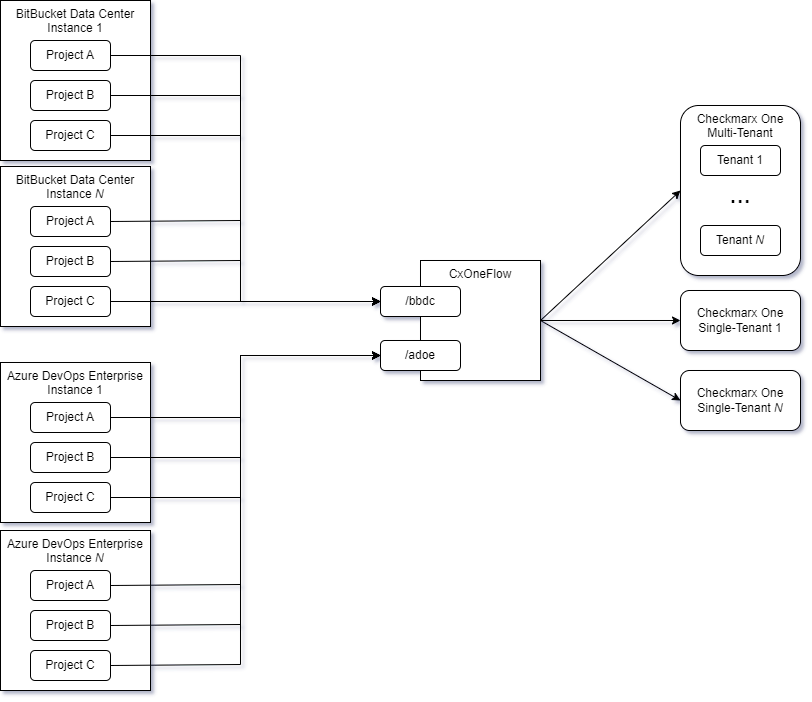
\includegraphics[width=\textwidth]{graphics/cxoneflow-deployment.png}
    \caption{\cxoneflow Deployment Diagram}
    \label{fig:cxoneflow-deployment}
\end{figure}

\section{Webhook Deployment Topology}

The goal of any \cxoneflow deployment is to enable webhook event delivery for a
large number of code repositories without a significant amount of effort.  Each 
SCM has several webhook deployment topologies that can be utilized to allow
deployment with the most minimal amount of effort. External factors can influence
what would be considered the most minimal amount of effort.

There are many factors that should be considered when considering the deployment
approach.  In some cases, some of the SCM webhook deployment capabilities may
not be utilized based on other considered factors.  Some of the
other factors to consider can include:

\begin{itemize}
    \item Administrative control of one or more SCM instances.
    \item Administrative control of multiple organizations in an SCM instance.
    \item Existing SCM integrations.
    \item Repository usage patterns that align with multiple development teams and Software Development Lifecycles.
\end{itemize}

This section is intended to provide a brief overview of the supported SCM repository organization topologies.
This overview is not comprehensive; a deeper look into your organization's SCMs may be required
to understand the full scope of deployment work.

The tool \extlink{https://github.com/checkmarx-ts/cxone-flow-audit}{cxone-flow-audit} has been
developed to assist in automating and auditing large scale deployments in some scenarios.  As
of the writing of this manual, the capabilities are limited to Azure DevOps.  As time progresses,
more deployment assistance capabilities will be added.


\subsection{BitBucket Data Center Topology}

BitBucket Data Center uses one or more \textbf{Project} logical unit to separate repositories
into logical groups.  Webhooks can be deployed at the \textbf{Project} scope; any changes
to a repository contained in a configured \textbf{Project} will emit webhook events.

Configuration of webhooks at the \textbf{Project} scope is generally the preferred
method of webhook deployment for BitBucket Data Center.

Webhooks can be deployed at the scope of each \textbf{Repository} if desired.  The number of repositories
in a large enterprise generally makes deployment at the \textbf{Repository} scope useful
only for testing purposes.

\subsection{Azure DevOps Topology}

Azure DevOps Enterprise (on-premise) uses one or more \textbf{Collection} logical units to separate
repositories into logical groups.  A \textbf{Collection} in Azure DevOps Enterprise 
corresponds to a Azure DevOps Cloud \textbf{Organization} in that the \textbf{Organization} is a logical unit 
that separates repositories into logical groups. Web hook deployments are not available at this scope.

In each \textbf{Collection} or \textbf{Organization}, zero or more \textbf{Project} logical
units establish the next level of repository organization.  Each \textbf{Project} will 
have one or more \textbf{Repository} units that will contain code that should be scanned.  Webhooks
can be deployed at this scope; each \textbf{Repository} in the configured \textbf{Project} logical unit
will emit webhook events when Service Hooks have been configured in the \textbf{Project} to
deliver webhook events to \cxoneflow.

Configuration of Service Hooks at the \textbf{Project} scope is generally the preferred
method of webhook deployment for Azure DevOps.

Webhooks can be deployed at the scope of each \textbf{Repository} if desired.  The number of repositories
in a large enterprise generally makes deployment at the \textbf{Repository} scope useful
only for testing purposes.

\subsection{GitHub Topology}

GitHub uses one or more \textbf{Organization} logical units to separate zero or more
repositories into logical groupings. Each GitHub user is also a limited variation of an
\textbf{Organization} in that a user account is also a logical unit that can have
associated repositories.  Webhook configurations can be deployed at this scope.
When webhooks are deployed at the \textbf{Organization} scope, events
will be emitted for all repositories within the \textbf{Organization} logical unit.

Configuration of webhooks at the \textbf{Organization} scope is generally the preferred
method of webhook deployment for GitHub.

A \textbf{GitHub App} can be created that functions as a webhook deployment template.
The \textbf{GitHub App} can be deployed at the \textbf{Organization} scope using the
GitHub user interface.  This is the preferred method of defining and executing the webhook deployment.

Webhooks can be deployed at the scope of each \textbf{Repository} if desired.  The number of repositories
in a large enterprise generally makes deployment at the \textbf{Repository} scope useful
only for testing purposes.  

\subsection{Gitlab Topology}

Each Gitlab on-premise, self-hosted instance has a system-wide Service Hook configuration where webhook
configurations for \cxoneflow can be deployed.  When webhooks are deployed at this scope, 
all repositories regardless of location in the Gitlab topology will send webhook events to \cxoneflowns. 

Configuration of webhooks using the system-wide scope is generally the preferred
method of webhook deployment for Gitlab.  This is only available for Gitlab on-premise,
self-hosted instances.

All variations of Gitlab have zero or more \textbf{Group} and/or \textbf{Repository} logical units
at the root of the topology.  Each \textbf{Group} logical unit can also hold zero or more
\textbf{Group} and/or \textbf{Repository} units.  Webhook configuration at the \textbf{Group}
scope in groups closest to the root of the topology are generally the preferred
method of webhook deployment for Gitlab.  Deployment of webhook configurations at lower
group scopes should be avoided.

Webhooks can be deployed at the scope of each \textbf{Repository} if desired.  The number of repositories
in a large enterprise generally makes deployment at the \textbf{Repository} scope useful
only for testing purposes.
